\documentclass[10pt,letterpaper,twocolumn]{article}

\usepackage[T1]{fontenc}
\usepackage{lmodern}
\usepackage[margin=0.62in,columnsep=0.27in]{geometry}
\usepackage{amsmath,amssymb,mathtools,bm}
\usepackage{array,booktabs,tabularx}
\usepackage{graphicx}
\usepackage{xcolor}
\usepackage{enumitem}
\usepackage{microtype}
\usepackage{fancyhdr}
\usepackage{hyperref}
\usepackage{needspace}

\graphicspath{{figures/}}

% The user-local tools/array package is newer than the available LaTeX kernel.
\makeatletter
\def\vcenter@text{\vbox}
\makeatother

\definecolor{navy}{HTML}{17365D}
\definecolor{blue}{HTML}{2B6CB0}
\definecolor{pale}{HTML}{F3F7FB}
\definecolor{paleblue}{HTML}{EAF2FA}
\definecolor{green}{HTML}{2F6B4F}
\definecolor{palegreen}{HTML}{EDF7F1}
\definecolor{brick}{HTML}{9B2C2C}
\definecolor{palered}{HTML}{FFF1F1}
\definecolor{muted}{HTML}{4A5568}

\hypersetup{
  colorlinks=true,
  linkcolor=navy,
  urlcolor=blue,
  pdftitle={Addendum: Mixed-Moment Failure and Joint Electron--Phonon Correction},
  pdfauthor={Holstein-dimer stability calculation}
}

\pagestyle{fancy}
\fancyhf{}
\fancyhead[L]{\footnotesize Holstein-dimer stability addendum}
\fancyhead[R]{\footnotesize Mixed moments and joint correction}
\fancyfoot[C]{\thepage}
\renewcommand{\headrulewidth}{0.3pt}

\setlength{\parindent}{0pt}
\setlength{\parskip}{3.0pt plus 0.5pt}
\setlist{nosep,leftmargin=*,topsep=2pt}
\renewcommand{\arraystretch}{1.10}
\newcolumntype{Y}{>{\raggedright\arraybackslash}X}

\newcommand{\R}{\mathbb R}
\newcommand{\C}{\mathbb C}
\newcommand{\I}{\mathbb I}
\newcommand{\ii}{\mathrm i}

\newcommand{\tracebox}[2]{%
  \par\smallskip
  \noindent\begin{minipage}{\columnwidth}
    {\color{#1}\rule{\columnwidth}{1.1pt}}\par\vspace{-1pt}
    \small\textbf{\color{#1}#2}\par\smallskip\color{black}
}
\newcommand{\closetracebox}{%
  \par\vspace{1pt}{\color{navy!35}\rule{\columnwidth}{0.35pt}}
  \end{minipage}\par\smallskip
}
\newcommand{\segmenthead}[1]{%
  \Needspace{5\baselineskip}%
  \par\medskip{\color{navy}\large\bfseries #1}\par
  \vspace{-2pt}{\color{navy}\rule{\columnwidth}{0.7pt}}\par\smallskip
}
\newcommand{\conceptbreak}{%
  \par\medskip\noindent
  {\color{black!30}\rule{\columnwidth}{0.35pt}}%
  \par\medskip
}

\newcommand{\RunTime}{1000}
\newcommand{\RunMinG}{2.06367\times10^{-5}}
\newcommand{\RunMinB}{2.06469\times10^{-5}}
\newcommand{\RunMinRho}{0.0239455}
\newcommand{\RunMaxRho}{0.976055}
\newcommand{\RunMaxX}{2.09860}
\newcommand{\RunMaxTrace}{8.78\times10^{-17}}
\newcommand{\RunEnergyDrift}{5.03\times10^{-6}}
\newcommand{\RunMaxCorrection}{0.345567}

\begin{document}
\raggedbottom
\setcounter{page}{15}

\twocolumn[
\begin{center}
  {\color{navy}\LARGE\bfseries Addendum}\par\vspace{3pt}
  {\Large Mixed-Moment Failure and the Joint Electron--Phonon Correction}\par\vspace{5pt}
  {\small Continuation of \emph{What We Actually Built}, 1 August 2026}
\end{center}
\vspace{3pt}
\hrule
\vspace{7pt}
]

\segmenthead{A. Problem Reconstruction}

The restricted dimer equations evolve the real coordinate vector
\(x^{(13)}(t)=(x_0(t),\ldots,x_{12}(t))\in\R^{13}\).  Its four physical
blocks are
\begin{center}
\small
\begin{tabularx}{\columnwidth}{@{}c Y Y@{}}
\toprule
\(j\) & stored coordinates & physical content\\
\midrule
0--2 & \(\Delta n,\Re\rho_{01},\Im\rho_{01}\) & electronic population imbalance and coherence\\
3--4 & \(\Re\Delta B,\Im\Delta B\) & relative coherent phonon displacement and momentum\\
5--6 & \(n_{\rm ph},\rho_{\rm ph}\) & normal phonon population and cross-mode coherence\\
7--12 & six real combinations of \(C\) & electron--phonon fluctuation correlations\\
\bottomrule
\end{tabularx}
\end{center}
Here \(\Delta B=B_0-B_1\), and \(C\) is the connected electron--phonon
correlation.  The first three entries alone form the electronic Bloch block:
\[
\rho=
\begin{pmatrix}
(1+\Delta n)/2&\Re\rho_{01}+\ii\Im\rho_{01}\\
\Re\rho_{01}-\ii\Im\rho_{01}&(1-\Delta n)/2
\end{pmatrix}.
\]
Its Bloch vector is
\[
\bm r=(2\Re\rho_{01},-2\Im\rho_{01},\Delta n).
\]
The remaining ten entries carry phonon and electron--phonon information.

Define the amplitude diagnostic and its maximizing coordinate by
\[
\begin{aligned}
a_{13}(t)
&=\lVert x^{(13)}(t)\rVert_\infty
=\max_{0\leq j\leq12}|x_j(t)|,\\
j_\star(t)
&\in\underset{0\leq j\leq12}{\operatorname{argmax}}|x_j(t)|.
\end{aligned}
\tag{R1}
\]
The absolute value detects growth in either sign.  The maximum is the upper
envelope of all thirteen traces, so it supplies one solver stopping statistic
without selecting a failing component in advance.  The identity of that
component is recovered from \(j_\star(t)\), which may change with time.
For the pinned strong-coupling case, the uncorrected equations produced the
declared amplitude divergence
\[
a_{13}(t)\geq10^4
\quad\text{at}\quad
t\simeq130.47\,t_{\rm hop}^{-1}.
\tag{R2}
\]
Here \(t_{\rm hop}\) is the electronic hopping energy and
\(t_{\rm hop}^{-1}\) is the time unit.  The matched weak-coupling calculation
remained bounded through \(t=140\,t_{\rm hop}^{-1}\); its largest sampled
value was \(a_{13}=0.6044\).

\Needspace{5\baselineskip}
At the strong threshold, the maximizing coordinate is
\[
j_\star=10,
\qquad x_{j_\star}=\Delta\operatorname{Im}^{-}.
\]
This variable is an imaginary symmetry combination of the electron--phonon
correlation \(C\).

Figure~40 in the source notes supplied the motivating energy and occupation
failure near \(t\approx105.3\) in its plotted time coordinate.  That earlier
plot supplied the question that initiated the reconstruction.  The present
calculation begins from the archived equations, parameters, and initial state;
it does not extract trajectory data from the plotted curves.  Equation~(R2) is
therefore an independent restricted-equation reproduction.  The two
calculations share the strong-coupling parameters and late-time instability,
while their plotted quantities and event times differ.  The result at
\(t=130.47\) reproduces the instability class rather than the individual
Figure~40 curves.

\textbf{How the failure was reproduced.}
We transcribed the relevant archived matrix equations, specialized their
electronic and phonon indices to the driven two-site Holstein dimer, applied
the pinned pulse and initial condition, formed the corresponding
thirteen-coordinate right-hand side, and integrated that right-hand side
without a matrix correction.  The calculation therefore followed
\begin{center}
\small
archived matrix equations
\(\longrightarrow\) two-site Holstein specialization
\(\longrightarrow\) restricted coordinate velocity
\(\longrightarrow\) uncorrected propagation
\(\longrightarrow a_{13}(t)\).
\end{center}

The pulse is the difference between the two driven on-site energies,
\[
V(t)=2V_0\sin\!\left(\frac{\pi t}{4}\right)
\exp\!\left[-\frac12\left(\frac{t}{\tau}\right)^2\right],
\tag{R3}
\]
with \(t_{\rm hop}=V_0=\tau=1\) in the dimensionless implementation.  The
ratios
\(\gamma=\omega_{\rm ph}/t_{\rm hop}=0.5\) and
\(\lambda_{\rm ep}=2g^2/(t_{\rm hop}\omega_{\rm ph})\) fix the phonon
frequency \(\omega_{\rm ph}\) and local coupling \(g\).  The strong trace uses
\(\lambda_{\rm ep}=1.5\); the matched weak trace changes only this value to
\(0.5\).  Both start from
\(x^{(13)}(0)=(0,\tfrac12,0,\ldots,0)\): the Hartree--Fock electronic
one-body density has \(\Re\rho_{01}=1/2\), and every retained phonon and
electron--phonon correlation coordinate starts at zero.  Fixed-step RK4 with
\(\Delta t=0.01\,t_{\rm hop}^{-1}\) records Eq.~(R1) at every step.

\begin{center}
\includegraphics[width=\columnwidth]{trajectory_max_abs.pdf}

\parbox{0.96\columnwidth}{\scriptsize
\textbf{Uncorrected restricted trajectories.}
The strong trace reaches the declared \(10^4\) threshold near
\(t=130.47\,t_{\rm hop}^{-1}\).  With the same pulse, phonon ratio, initial
condition, solver, and horizon, the weak trace remains bounded through
\(t=140\,t_{\rm hop}^{-1}\).}
\end{center}

\textbf{Why the 31-coordinate calculation followed.}
The restricted calculation reproduces the late amplitude symptom.  The
archived matrix right-hand side also generates matrix directions outside
that thirteen-coordinate slice.  Retaining all 31 independent real entries
of \((\rho,B,N,A,C)\) captures the complete generated matrix velocity in the
tested dimer sector and permits physical matrix conditions to be evaluated
along the trajectory.  Here \(\rho\) is the electronic one-body density,
\(B\) contains the coherent phonon amplitudes, \(N\) and \(A\) contain
centered phonon second moments, and \(C\) contains connected
electron--phonon correlations.
Once this full velocity is explicit, Section~B compares it with the exact
contracted velocity and decomposes the resulting \(C\)-block defect into its
operator contributions.  Thus the 31-coordinate representation enables the
subsequent term attribution as well as the matrix-condition diagnosis.

The first such diagnostic is the bosonic moment matrix
\[
M_{\rm B}(t)=
\begin{pmatrix}
N(t)^{\mathsf T}&A(t)^\ast\\
A(t)&\I_2+N(t)
\end{pmatrix},
\tag{R4}
\]
where \(N\) and \(A\) are the normal and anomalous centered phonon
second-moment matrices, and \(\I_2\) is the two-dimensional identity.  A
physically representable pair \((N,A)\) requires
\(M_{\rm B}\succeq0\), meaning that every eigenvalue is nonnegative.  The
31-coordinate uncorrected trajectory reaches this boundary when its smallest
eigenvalue obeys
\[
\lambda_{\min}\!\left(M_{\rm B}\right)=0
\quad\text{at}\quad
t=1.48695622\,t_{\rm hop}^{-1}.
\tag{R5}
\]
Equation~(R5) is the boundary of the positive-semidefinite cone: continuation
to \(\lambda_{\min}(M_{\rm B})<0\) leaves the set of representable bosonic
second moments.  This upstream physical failure occurs long before the
restricted amplitude threshold at \(t=130.47\,t_{\rm hop}^{-1}\).  The
thirteen-coordinate run reproduces the original symptom; the 31-coordinate
run identifies its earlier physical precursor.

\tracebox{brick}{Correction to the printed Section 3}
Printed Eq.~(J3) constrained the electronic density and bosonic moment matrix
as three separate positive-semidefinite blocks.  Its completed
\(t=1000\,t_{\rm hop}^{-1}\) trajectory remains evidence that those separate
blocks can be stabilized under the printed composite regularization.  Applied
to the raw archive closure, its thirteen correction coordinates became
infeasible near \(t=28.57\).  Allowing all 31 velocity coordinates restored
optimization feasibility and still constrained only the separate blocks.  The
electron--phonon correlation \(C\) occupies an off-diagonal block of a stronger
joint moment matrix.  The all-coordinate separate-block run was stopped at
\(t=320\), where that joint matrix had eigenvalues including \(-2.621\) and
\(-1.803\).
Consequently, the printed claim of full physicality is replaced by the joint
construction.  The printed equations and coordinate maps remain valid
premises for its derivation.
\closetracebox

\segmenthead{B. What failed first in the 31-coordinate closure}

Recall the retained matrix state
\(X=(\rho,B,N,A,C)\), its coordinate extraction
\(\mathcal R:X\mapsto x\in\R^{31}\), and the closure velocity
\(f(t,x)=\Pi F(t,\mathcal E(x))\).  An independently propagated truncated
Holstein-dimer state \(\lvert\Psi_{\rm ex}(t)\rangle\) supplies an exact
reference at the same state and time:
\[
\lvert\Psi_{\rm ex}(t)\rangle
\xrightarrow{\text{expectation values}}
X_{\rm ex}(t)
\xrightarrow{\mathcal R}
x_{\rm ex}(t).
\tag{X1}
\]
The Hamiltonian commutator differentiates each expectation value, producing
\(\dot X_{\rm ex}(t)\) without a trajectory finite difference.  The closure
derivative and exact contracted derivative can therefore be evaluated on the
same retained data:
\[
\begin{aligned}
d_{\rm cl}(t)&=f\bigl(t,x_{\rm ex}(t)\bigr),\\
d_{\rm ex}(t)&=\mathcal R\dot X_{\rm ex}(t),\\
r(t)&=d_{\rm cl}(t)-d_{\rm ex}(t).
\end{aligned}
\tag{X2}
\]
Here \(r(t)\in\R^{31}\) is the derivative defect.  For a short interval
\(\Delta t\), the two predictions differ by
\[
x_{\rm cl}(t+\Delta t)-x_{\rm ex}(t+\Delta t)
=\Delta t\,r(t)+O(\!\Delta t^2).
\tag{X3}
\]
Thus the block containing the first nonzero entries of \(r\) identifies the
first locally incorrect retained velocity.

The exact ground-state contractions at
\(\lambda=1.5\), \(\gamma=0.5\), and phonon cutoff 16 have energy
\(-3.7753265535\,t_{\rm hop}\).  Their second-order-closure velocity has
undriven initial residual norm \(0.3714\).
Subtracting that constant residual was tested as an initialization repair.
At \(t=0.5\), the residual-subtracted comparison gives
\[
\begin{array}{@{}l r@{}}
\toprule
\text{derivative block} & \ell_2\text{ defect}\\
\midrule
\rho,B,N,A\ \text{together} & <7\times10^{-6}\\
C & 4.8511144\times10^{-2}\\
\text{all 31 coordinates} & 4.8511145\times10^{-2}\\
\bottomrule
\end{array}
\tag{X4}
\]
The equality of the last two scales localizes the first defect in \(\dot C\).
Cutoffs 12, 16, and 20 give total defects \(0.04610\), \(0.04851\), and
\(0.04860\), respectively, thereby excluding cutoff 16 as the leading cause.

\conceptbreak
\textbf{The exact operator split.}
Let \(O_{ij}=c_{j\uparrow}^\dagger c_{i\uparrow}\),
\(n_{r\uparrow}=c_{r\uparrow}^\dagger c_{r\uparrow}\), and
\(\delta X_r=\delta b_r+\delta b_r^\dagger\).  The exact interaction
contribution to \(\dot C^q_{ij}\) requests
\[
\begin{aligned}
Q^{qr}_{ij}
&=\left\langle
[O_{ij},n_{r\uparrow}]\,\delta X_r\,\delta b_q
\right\rangle,\\
Q^{qr}_{ij,0}
&=\left\langle[O_{ij},n_{r\uparrow}]\right\rangle
\left\langle\delta X_r\,\delta b_q\right\rangle,\\
K^{qr}_{ij}&=Q^{qr}_{ij}-Q^{qr}_{ij,0}.
\end{aligned}
\tag{X5}
\]
The product \(Q^{qr}_{ij,0}\) uses the retained electronic first moment and
phonon second moment.  Its connected remainder \(K^{qr}_{ij}\) records the
joint fluctuation left unexplained by that product and contributes
\[
\Delta\dot C^q_{K,ij}
=-\ii g\sum_{r=0}^{1}K^{qr}_{ij}.
\tag{X6}
\]

Two additional operator contributions enter at the same line.  Fixed
one-up-electron number gives the exact same-spin covariance
\[
\begin{aligned}
P^q_{ij}
&=\operatorname{Cov}(O_{ij},n_{q\uparrow})
=\delta_{iq}\rho_{qj}-\rho_{ij}\rho_{qq},\\
D^q_{ij}
&=\operatorname{Cov}(O_{ij},n_{q\downarrow})\\
&=\langle O_{ij}n_{q\downarrow}\rangle
-\rho_{ij}\langle n_{q\downarrow}\rangle .
\end{aligned}
\tag{X7}
\]
Archive Eq.~(14d) separately factorizes the two products inside the
same-spin commutator.  Replacing that result by \(P^q_{ij}\) restores the
exact Pauli multiplication rule, including
\([n_{i\uparrow},n_{r\uparrow}]=0\).  The opposite-spin covariance
\(D^q_{ij}\) is absent from the 31 retained coordinates.  Together with the
finite-cutoff commutator remainder \(R_{\rm cut}\), these objects give the
source-faithful identity
\[
\boxed{
\dot C_{\rm ex}
=\dot C_{31}
+\Delta\dot C_K
+\Delta\dot C_P
+\Delta\dot C_D
+R_{\rm cut}.}
\tag{X7a}
\]
Here \(\Delta\dot C_P\) replaces the archive Pauli source by its exact
fixed-sector value, and
\(\Delta\dot C^q_{D,ij}=-\ii gD^q_{ij}\).

Between \(t=0\) and \(t=0.5\), the respective source-vector changes have
14-coordinate norms \(0.048149\), \(0.007873\), \(0.005737\), and
\(8.68\times10^{-6}\).  The vectors partially cancel.  The previous value
\(0.04797\) grouped the Pauli repair into an effective archive \(K\), and the
previous \(9.0\times10^{-5}\) same-spin attribution is superseded by this
operator-level split.  The genuine evolving \(K\) remains the largest
individual source.

The retained feedback carries the resulting error into the other moments:
\[
\begin{aligned}
\dot C\ \text{defect}
&\longrightarrow(\dot\rho,\dot N,\dot A)\ \text{defects}\\
&\longrightarrow\text{loss of representability}.
\end{aligned}
\tag{X7b}
\]
A constant subtraction matches the missing contribution at one time.  The
subtracted value remains fixed as Eqs.~(X6)--(X7a) evolve under the drive.

\segmenthead{C. The joint Gram matrix that detects the loss}

The printed admissible set tested three separate matrices.  Denote it by
\[
\mathcal P_{\rm s}
=\{x:\rho\succeq0,\ \I_2-\rho\succeq0,\ M_{\rm B}\succeq0\}.
\tag{X8}
\]
To couple those marginal conditions to \(C\), define the Pauli expectation
\(r_a=\operatorname{Tr}(\rho\sigma_a)\) and its centered operator
\(\delta\sigma_a=\sigma_a-r_a\I_2\), where
\(a\in\{x,y,z\}\).  Combine four centered phonon operators and three
centered electronic operators into
\[
Y=(\delta b_0,\delta b_1,\delta b_0^\dagger,\delta b_1^\dagger,
\delta\sigma_x,\delta\sigma_y,\delta\sigma_z).
\tag{X9}
\]
The \(7\times7\) Gram matrix of these operator-valued directions is
\[
\mathcal G_{ab}=\langle Y_a^\dagger Y_b\rangle,
\qquad
z^\dagger\mathcal Gz
=\left\langle
\Bigl(\sum_a z_aY_a\Bigr)^\dagger
\Bigl(\sum_bz_bY_b\Bigr)
\right\rangle\geq0.
\tag{X10}
\]
Every physical state therefore requires \(\mathcal G\succeq0\).

The retained moments construct every block explicitly.  Define
\[
\begin{aligned}
c_{qa}&=\operatorname{Tr}(C^q\sigma_a),
&Z(C)&=\begin{pmatrix}c^\ast\\c\end{pmatrix},\\
E_{ab}(\rho)
&=\operatorname{Tr}(\rho\sigma_a\sigma_b)-r_ar_b,
&c&=(c_{qa})\in\C^{2\times3}.
\end{aligned}
\tag{X11}
\]
Then
\[
\boxed{
\mathcal G(\rho,N,A,C)
=\begin{pmatrix}
M_{\rm B}(N,A)&Z(C)\\
Z(C)^\dagger&E(\rho)
\end{pmatrix}\succeq0.}
\tag{X12}
\]
The diagonal blocks store bosonic and electronic fluctuation moments.  The
off-diagonal block stores their cross-correlation.  In the interior
\(M_{\rm B}\succ0\), block elimination gives the Schur-complement form
\[
\mathcal G\succeq0
\quad\Longleftrightarrow\quad
M_{\rm B}\succ0,
\quad
E(\rho)-Z(C)^\dagger M_{\rm B}^{-1}Z(C)\succeq0.
\tag{X13}
\]
The second matrix subtracts the electronic variance already consumed by the
mixed correlation.  Separate positivity leaves the magnitude of \(Z(C)\)
unbounded relative to the two marginal variances; Eq.~(X13) imposes the
operator Cauchy--Schwarz relation joining all three blocks.

Fixed particle number adds one exact equality.  From the definition
\(C^q_{ij}=\langle\delta b_q(c_j^\dagger c_i-\rho_{ij})\rangle\),
\[
\operatorname{Tr}C^q
=\left\langle\delta b_q
\left(\sum_i n_i-\sum_i\rho_{ii}\right)\right\rangle=0.
\tag{X14}
\]
This gives the two separate identities
\(\operatorname{Tr}C^0=\operatorname{Tr}C^1=0\), which are stronger than
equality of the two traces alone.  They remain linear constraints:
\[
\operatorname{Tr}(\alpha C^q)=0
\quad\text{for every scalar }\alpha.
\tag{X14a}
\]
Meanwhile \(Z(\alpha C)=\alpha Z(C)\), so sufficiently large \(|\alpha|\)
can violate the Schur inequality in Eq.~(X13) while Eq.~(X14a) remains exact.
For each \(q\), trace zero fixes one complex linear combination of the four
entries of \(C^q\).  Joint positivity quantifies over every coefficient vector
\(z\) in Eq.~(X10), and therefore constrains every centered electron--phonon
operator combination assembled from those entries.  The trace identities
preserve fixed-number structure; joint positivity additionally bounds the
correlation magnitude relative to the electronic and bosonic variances.
Hence the stronger retained-moment set is
\[
\boxed{
\mathcal P_{\rm j}
=\{x\in\mathcal P_{\rm s}:\mathcal G(x)\succeq0,
\ \operatorname{Tr}C^q=0\ (q=0,1)\}
\subset\mathcal P_{\rm s}.}
\tag{X15}
\]

On the raw archive closure initialized by the exact cutoff-16 contractions,
\(\lambda_{\min}(\mathcal G)\) first reaches zero at
\[
t=0.1607116782\,t_{\rm hop}^{-1}.
\tag{X16}
\]
At that same state,
\(\lambda(\rho)=(0.10380,0.89620)\) and
\(\lambda_{\min}(M_{\rm B})=1.8890\times10^{-3}\).  The trajectory has
therefore left \(\mathcal P_{\rm j}\) while remaining inside every separately
tested cone.  The exact truncated-Hamiltonian trajectory retains
\(\mathcal G\succeq0\).  The raw closure also assigns
\(\operatorname{Im}\operatorname{Tr}\dot C^q=-0.0593937\) to the exact
initial contractions, directly violating the tangent form of Eq.~(X14).

\segmenthead{D. Explicit 31-coordinate velocity lift}

The correction variable \(w=(w_0,\ldots,w_{30})\in\R^{31}\) uses the same
coordinate order as printed Eq.~(R7).  It is a tangent vector: its matrix lift
adds a velocity and therefore omits the constant one-half terms in the affine
state reconstruction.  The electronic and coherent-phonon lifts are
\[
\begin{aligned}
\Delta\dot\rho(w)&=
\begin{pmatrix}
w_0/2&w_1+\ii w_2\\w_1-\ii w_2&-w_0/2
\end{pmatrix},\\[2pt]
\Delta\dot B(w)&=
\begin{pmatrix}w_3+\ii w_4\\w_5+\ii w_6\end{pmatrix}.
\end{aligned}
\tag{X17}
\]
The normal and anomalous second-moment lifts are
\[
\begin{aligned}
\Delta\dot N(w)&=
\begin{pmatrix}
w_7&w_9+\ii w_{10}\\w_9-\ii w_{10}&w_8
\end{pmatrix},\\
\Delta\dot A(w)&=
\begin{pmatrix}
w_{11}+\ii w_{12}&w_{15}+\ii w_{16}\\
w_{15}+\ii w_{16}&w_{13}+\ii w_{14}
\end{pmatrix}.
\end{aligned}
\tag{X18}
\]
Their structured bosonic lift follows by differentiating printed Eq.~(12):
\[
\Delta\dot M_{\rm B}(w)=
\begin{pmatrix}
\Delta\dot N(w)^{\mathsf T}&\Delta\dot A(w)^\ast\\
\Delta\dot A(w)&\Delta\dot N(w)
\end{pmatrix}.
\tag{X19}
\]
The identity block contributes zero derivative.

The first two correlation coordinates form the shared trace.  The complete
correlation lift is
{\scriptsize
\[
\begin{aligned}
\Delta\dot C^0(w)&=
\begin{pmatrix}
\frac{w_{17}+\ii w_{18}+w_{19}+\ii w_{20}}2&w_{21}+\ii w_{22}\\
w_{23}+\ii w_{24}&\frac{w_{17}+\ii w_{18}-w_{19}-\ii w_{20}}2
\end{pmatrix},\\[3pt]
\Delta\dot C^1(w)&=
\begin{pmatrix}
\frac{w_{17}+\ii w_{18}+w_{25}+\ii w_{26}}2&w_{27}+\ii w_{28}\\
w_{29}+\ii w_{30}&\frac{w_{17}+\ii w_{18}-w_{25}-\ii w_{26}}2
\end{pmatrix}.
\end{aligned}
\tag{X20}
\]
}
These displays contain all 31 independent correction coordinates.  They add
no matrix degree of freedom beyond the established Hermitian, symmetric, and
shared-trace relations.

To obtain the joint matrix velocity, define
\(\Delta r_a=\operatorname{Tr}(\Delta\dot\rho\,\sigma_a)\) and
\(\Delta c_{qa}=\operatorname{Tr}(\Delta\dot C^q\sigma_a)\).  Differentiating
Eqs.~(X11)--(X12) gives
\[
\begin{aligned}
(\Delta\dot E)_{ab}
&=\operatorname{Tr}(\Delta\dot\rho\,\sigma_a\sigma_b)
-\Delta r_a r_b-r_a\Delta r_b,\\
\Delta\dot Z&=\begin{pmatrix}\Delta c^\ast\\\Delta c\end{pmatrix},\\
\Delta\dot{\mathcal G}(w)
&=\begin{pmatrix}
\Delta\dot M_{\rm B}(w)&\Delta\dot Z(w)\\
\Delta\dot Z(w)^\dagger&\Delta\dot E(w)
\end{pmatrix}.
\end{aligned}
\tag{X21}
\]
Equation~(X21) is the structured lift used by the joint barrier.  It shows
entry by entry how a 31-real-coordinate correction changes a
\(7\times7\) Hermitian moment-matrix velocity.

\segmenthead{E. Corrected Semidefinite Velocity}

At one right-hand-side evaluation, let \(\dot x_0=f(t,x)\) be the archive
closure velocity, and reconstruct \(\dot\rho_0\) and
\(\dot{\mathcal G}_0\) from it.  The barrier rate \(\beta=5\) controls how
quickly an interior margin is restored, the safety margin is
\(h_\star=10^{-5}\), and \(I_d\) is the \(d\times d\) identity.  These
objects form the three raw barrier matrices
{\footnotesize
\[
\begin{aligned}
M_{0,\rho}^{-}
&=\dot\rho_0+\beta(\rho-h_\star I_2),
&\Delta M_{\rho}^{-}(w)&=\Delta\dot\rho(w),\\
M_{0,\rho}^{+}
&=-\dot\rho_0+\beta(I_2-\rho-h_\star I_2),
&\Delta M_{\rho}^{+}(w)&=-\Delta\dot\rho(w),\\
M_{0,\mathcal G}
&=\dot{\mathcal G}_0+\beta(\mathcal G-h_\star I_7),
&\Delta M_{\mathcal G}(w)&=\Delta\dot{\mathcal G}(w).
\end{aligned}
\tag{X21a}
\]
}
The superscripts \(-\) and \(+\) label the lower boundary
\(\rho\succeq0\) and upper boundary \(I_2-\rho\succeq0\).  The subscript
\(0\) denotes the uncorrected archive velocity; each \(\Delta M(w)\) is the
change induced by the correction lift.  A negative eigenvalue of a raw
barrier matrix means that the uncorrected velocity violates the differential
barrier in that matrix direction.  The current matrix itself may still have
nonnegative eigenvalues, as Eq.~(X16) demonstrates for \(\mathcal G\) before
its later cone exit.

For one scalar matrix margin \(m(t)\), the same differential condition is
\[
\begin{aligned}
\dot m+\beta(m-h_\star)&\geq0,\\
m(t)&\geq h_\star+(m(0)-h_\star)e^{-\beta t}
\end{aligned}
\tag{X22}
\]
The boundary is the positive level \(m=h_\star\).  Substitution into the first
line gives \(\dot m\geq0\), so the velocity is tangent to the boundary or
directed toward larger \(m\).  When \(m>h_\star\), the condition permits
\(\dot m<0\) down to \(-\beta(m-h_\star)\); the available margin therefore
allows controlled motion toward the boundary.

The correction is the minimum-norm solution
{\footnotesize
\[
\begin{aligned}
\underset{w\in\R^{31}}{\operatorname{minimize}}\quad
&\tfrac12\lVert w\rVert_2^2\\
\text{subject to}\quad
&\dot\rho_0+\Delta\dot\rho(w)
+\beta(\rho-h_\star I_2)\succeq0,\\
&-\dot\rho_0-\Delta\dot\rho(w)
+\beta(I_2-\rho-h_\star I_2)\succeq0,\\
&\dot{\mathcal G}_0+\Delta\dot{\mathcal G}(w)
+\beta(\mathcal G-h_\star I_7)\succeq0,\\
&\dot s_0+w_{17}+\ii w_{18}+\beta s=0,\\
&\nabla_xE(x)^{\mathsf T}w=0.
\end{aligned}
\tag{X23}
\]
}
The shared correlation trace is \(s=\operatorname{Tr}C^q\).  Its raw rate is
\(\dot s_0\), and the correction coordinates \(w_{17}+\ii w_{18}\) add the
trace-rate correction.  The complex fourth line is therefore two real
equalities and gives
\[
\dot s_{\rm c}=\dot s_0+w_{17}+\ii w_{18}=-\beta s,
\qquad
s(t)=s(0)e^{-\beta t}.
\tag{X23a}
\]
Equation~(X14) derives \(s=0\) from fixed particle number.  An initial shared
trace \(s(0)=0\) consequently remains zero; a small numerical trace error
decays at rate \(\beta\).  The last line makes the added velocity
energy-neutral.  Using printed Eq.~(J0), its fully expanded coordinate form is
{\scriptsize
\[
\begin{aligned}
0={}&2g(\Re B_0-\Re B_1)w_0-4t_{\rm hop}w_1\\
&+(2\omega_{\rm ph}\Re B_0+4g\rho_{00})w_3
+2\omega_{\rm ph}\Im B_0w_4\\
&+(2\omega_{\rm ph}\Re B_1+4g\rho_{11})w_5
+2\omega_{\rm ph}\Im B_1w_6\\
&+\omega_{\rm ph}(w_7+w_8)
+4gw_{17}+2gw_{19}-2gw_{25}.
\end{aligned}
\tag{X24}
\]
}
The affine state map already fixes \(\operatorname{Tr}\rho=1\), and
Eq.~(X17) gives \(\operatorname{Tr}\Delta\dot\rho(w)=0\) identically.  Its
displayed matrix forms likewise preserve Hermiticity of \(\rho,N\) and
symmetry of \(A\).  These structural relations are built into the lift;
Eq.~(X23) adds the positive-semidefinite inequalities, the correlation-trace
equality, and the energy row.

Let \(E_{\rm int}(x)\) denote the time-independent internal-energy functional
in printed Eq.~(J0).  Along the corrected velocity,
\[
\frac{dE_{\rm int}}{dt}
=\nabla_xE_{\rm int}^{\mathsf T}f(t,x)
+\nabla_xE_{\rm int}^{\mathsf T}w^\star.
\tag{X24a}
\]
The last equality in Eq.~(X23) sets only the second term to zero.  The first
term remains the energy transfer generated by the archive dynamics, including
the work delivered through the drive \(V(t)\).  The controller therefore adds
no instantaneous internal-energy flux and does not force the driven energy to
remain constant.  Every omitted coordinate in Eq.~(X24) has zero direct
coefficient in \(E_{\rm int}\).

The Euclidean objective measures the intervention in the displayed
31-coordinate scaling; a weighted coordinate metric would select a different
minimum-norm feasible velocity.

The corrected differential equation is
\[
\boxed{\dot x_{\rm c}=f(t,x)+w^\star(t,x).}
\tag{X25}
\]
It changes the velocity used to construct the next solver step while retaining
the current state.  Since
\(\lVert\dot x_{\rm c}-f(t,x)\rVert_2=\lVert w^\star\rVert_2\), the objective
selects the nearest feasible velocity in this coordinate metric.
Equation~(X25) thereby implements a continuous-time barrier correction.

\conceptbreak
\textbf{How the solve is executed.}
After satisfying the trace and energy equalities through an affine null-space
parameterization, the algorithm diagonalizes the three raw barrier matrices in
Eq.~(X21a).  Let \(M_0=M_0^\dagger\) denote the selected raw matrix and
\(\Delta M(w)\) its corresponding correction lift.  If its smallest
eigenvalue is negative, choose a normalized eigenvector \(v\) satisfying
\[
M_0v=\lambda v,
\qquad
v^\dagger v=1,
\qquad
\lambda=v^\dagger M_0v<0.
\tag{X25a}
\]
The scalar \(\lambda\) is the raw differential-barrier value in the direction
\(v\).  For the joint Gram matrix, the entries of \(v\) are the coefficients
of the centered-operator combination
\(O_v=\sum_a v_aY_a\), whose physical quadratic form is
\(v^\dagger\mathcal Gv=\langle O_v^\dagger O_v\rangle\).
The correction changes the velocity of this operator combination through
\(\Delta M(w)\).  A nonnegative barrier value
along \(v\) is the constraint
\[
v^\dagger\bigl(M_0+\Delta M(w)\bigr)v\geq0
\quad\Longleftrightarrow\quad
v^\dagger\Delta M(w)v\geq-v^\dagger M_0v,
\tag{X26}
\]
The structured lift is linear:
\[
\begin{aligned}
\Delta M(w)
&=\sum_{j=0}^{30}w_j\Delta M(e_j),\\
v^\dagger\Delta M(w)v
&=\sum_{j=0}^{30}w_j
\bigl[v^\dagger\Delta M(e_j)v\bigr].
\end{aligned}
\tag{X26a}
\]
Define the scalar response of this exposed mode to the \(j\)-th unit
correction by
\[
\begin{aligned}
a_j&:=v^\dagger\Delta M(e_j)v,\\
a&:=(a_0,\ldots,a_{30})\in\R^{31},\\
\phi_v(w)
&:=v^\dagger\bigl[M_0+\Delta M(w)\bigr]v
=\lambda+a^{\mathsf T}w,\\
\frac{\partial\phi_v}{\partial w_j}&=a_j.
\end{aligned}
\tag{X26b}
\]
Thus \(a_j\) is the sensitivity of the exposed barrier value to one unit of
the \(j\)-th correction coordinate.  Its sign selects which sign of \(w_j\)
raises the barrier value, and \(|a_j|\) measures how strongly that coordinate
changes the failing operator combination \(O_v\).  The vector \(a\) is normal
to the boundary hyperplane \(a^{\mathsf T}w=-\lambda\) in correction-coordinate
space.  Linearity follows from the linear matrix lift with \(v\) held fixed.

Positive semidefiniteness requires every matrix direction:
\[
\begin{aligned}
M_0+\Delta M(w)\succeq0
\quad\Longleftrightarrow\quad&\\[-0.8ex]
z^\dagger\bigl[M_0+\Delta M(w)\bigr]z&\geq0
\quad\text{for every }z.
\end{aligned}
\tag{X26c}
\]
Equation~(X26) enforces the condition for one exposed \(v\).  The corrected
matrix can have a different minimizing eigenvector, which supplies the next
half-space after diagonalization.

For one exposed mode with \(\lambda<0\) and \(a\neq0\), the origin
\(w=0\) violates \(a^{\mathsf T}w\geq-\lambda\).  Its nearest feasible point
follows from one Lagrange multiplier \(\mu\geq0\):
{\footnotesize
\[
\begin{aligned}
&\underset{w\in\R^{31}}{\operatorname{minimize}}
\ \frac12w^{\mathsf T}w
\quad\text{subject to}\quad a^{\mathsf T}w+\lambda\geq0,\\
&L(w,\mu)=\frac12w^{\mathsf T}w
-\mu(a^{\mathsf T}w+\lambda),\\
&\nabla_wL=w-\mu a=0
\quad\Longrightarrow\quad w=\mu a,\\
&a^{\mathsf T}w+\lambda=0
\quad\Longrightarrow\quad
\mu=\frac{-\lambda}{\lVert a\rVert_2^2},\\
&\boxed{w^\star=\frac{-\lambda}{\lVert a\rVert_2^2}a.}
\end{aligned}
\tag{X26d}
\]
}
The feasible set is the half-space on the inward side of the hyperplane
\(a^{\mathsf T}w=-\lambda\); Eq.~(X26d) is the Euclidean projection of the
origin onto that hyperplane along its normal \(a\).  The complete solve applies
this geometry after incorporating the equality constraints.

\conceptbreak
\textbf{Equality elimination by null-space coordinates.}
At one right-hand-side evaluation, collect the energy equality and the real
and imaginary correlation-trace equalities from Eq.~(X23) into
\(Lw=d\), where
{\footnotesize
\[
\begin{aligned}
L&=
\begin{pmatrix}
\nabla_xE_{\rm int}(x)^{\mathsf T}\\
e_{17}^{\mathsf T}\\
e_{18}^{\mathsf T}
\end{pmatrix}
\in\R^{3\times31},\\
d&=
\begin{pmatrix}
0\\
-\dot x_{0,17}-\beta x_{17}\\
-\dot x_{0,18}-\beta x_{18}
\end{pmatrix}
\in\R^3.
\end{aligned}
\tag{X26e}
\]
}
Here \(e_j\) is the \(j\)-th standard coordinate vector, so the last two rows
select the two real coordinates of \(s=\operatorname{Tr}C^q\).  A singular-value
decomposition of \(L\) returns its rank \(r\), the minimum-Euclidean-norm
particular solution \(w_{\rm p}=L^+d\), and an orthonormal basis
\(Z\in\R^{31\times(31-r)}\) for \(\ker L\):
\[
\begin{aligned}
Lw_{\rm p}&=d,&LZ&=0,\\
Z^{\mathsf T}Z&=I,&Z^{\mathsf T}w_{\rm p}&=0,\\
w&=w_{\rm p}+Zy,&y&\in\R^{31-r}.
\end{aligned}
\tag{X26f}
\]
Every \(y\) therefore produces a correction satisfying both equalities.  The
orthogonality in Eq.~(X26f) also gives
\[
\frac12\lVert w\rVert_2^2
=\frac12\lVert w_{\rm p}\rVert_2^2
+\frac12\lVert y\rVert_2^2.
\tag{X26g}
\]
The first term is fixed, so the remaining optimization minimizes
\(\lVert y\rVert_2\).  Consequently, the ``origin'' used by the numerical
projection is \(y=0\); in the original 31 coordinates it represents
\(w=w_{\rm p}\), the smallest correction already satisfying the equalities.

\conceptbreak
\textbf{One negative eigenvector produces one exact linear cut.}
Let \(\ell\in\{\rho^-,\rho^+,\mathcal G\}\) label one of the three barrier
sectors in Eq.~(X21a).  After Eq.~(X26f), its corrected barrier matrix is the
affine matrix-valued map
\[
B_\ell(y)
=M_{0,\ell}+\Delta M_\ell(w_{\rm p}+Zy).
\tag{X26h}
\]
At the current reduced point \(y^{(k)}\), diagonalization gives a normalized
negative mode
\[
B_\ell(y^{(k)})v=\lambda v,
\qquad \lambda<0.
\tag{X26i}
\]
Define its 31-coordinate response \(a_\ell(v)\) and reduced response \(n\) by
\[
\begin{aligned}
[a_\ell(v)]_j
&=v^\dagger\Delta M_\ell(e_j)v,\\
n&=Z^{\mathsf T}a_\ell(v).
\end{aligned}
\tag{X26j}
\]
Since \(B_\ell(y)\) is affine in \(y\), holding this exposed \(v\) fixed gives
the exact identity
\[
\begin{aligned}
v^\dagger B_\ell(y)v
&=\lambda+n^{\mathsf T}(y-y^{(k)}),\\
v^\dagger B_\ell(y)v\geq0
&\quad\Longleftrightarrow\quad
n^{\mathsf T}y\geq
n^{\mathsf T}y^{(k)}-\lambda.
\end{aligned}
\tag{X26k}
\]
Thus each negative eigenvector exposes one linear half-space containing every
semidefinite-feasible correction.  This relation is exact for that fixed
matrix direction; the repeated diagonalization is required because other
directions remain untested.

The full semidefinite feasible set is a \emph{spectrahedron}: the set of
reduced coordinates for which every affine matrix \(B_\ell(y)\) is positive
semidefinite.  Equation~(X26c) expresses it as the intersection of the
half-spaces generated by all normalized matrix directions.  A finite set of
exposed modes gives an outer polyhedral approximation to that spectrahedron.

\conceptbreak
\textbf{Cutting-plane quadratic program and direct fallback.}
After \(p\) cuts have been accumulated, the implemented subproblem is the
convex quadratic program
\[
\boxed{
\begin{aligned}
\underset{y\in\R^{31-r}}{\operatorname{minimize}}\quad
&\frac12y^{\mathsf T}y\\
\text{subject to}\quad
&n_i^{\mathsf T}y\geq c_i,
\qquad i=1,\ldots,p,
\end{aligned}}
\tag{X26l}
\]
where each \(n_i\) and \(c_i\) has the form in Eq.~(X26k).  SciPy's
Sequential Least Squares Programming optimizer, SLSQP, solves Eq.~(X26l) with
the exact objective gradient \(y\).  In this application it projects the
reduced origin onto the intersection of the accumulated half-spaces.  The
algorithm then reconstructs \(w=w_{\rm p}+Zy\), forms all three complete
barrier matrices, and diagonalizes them again:
\[
y^{(k)}
\longrightarrow B_\ell(y^{(k)})
\longrightarrow(\lambda,v)
\longrightarrow(n^{\mathsf T}y\geq c)
\longrightarrow y^{(k+1)}.
\tag{X26m}
\]
Previously generated cuts remain in Eq.~(X26l).  The cycle stops only when all
three complete matrices have minimum eigenvalue above the declared cone
tolerance.  This is the cutting-plane realization of the minimum-norm
semidefinite correction.

Near a degenerate boundary, two or more eigenvectors can exchange order and the
finite cutting-plane cycle can stall numerically.  The fallback asks SLSQP to
solve the complete spectral constraints directly:
\[
\begin{aligned}
\underset{y\in\R^{31-r}}{\operatorname{minimize}}\quad
&\frac12y^{\mathsf T}y\\
\text{subject to}\quad
&\lambda_m(B_\ell(y))\geq0
\quad\text{for every }\ell,m.
\end{aligned}
\tag{X26n}
\]
For a simple eigenvalue, the supplied derivative is the same exposed-mode
response,
\[
\frac{\partial\lambda_m(B_\ell(y))}{\partial y_j}
=v_m^\dagger
\frac{\partial B_\ell(y)}{\partial y_j}v_m.
\tag{X26o}
\]
The fallback begins from the cutting-plane result and verifies feasibility from
the complete matrices.  A separately requested direct solve also provides an
independent implementation check: at the exact cutoff-16 initial state its
correction norm agrees with the cutting-plane norm to relative tolerance
\(2\times10^{-7}\).

Both routes minimize the Euclidean norm of the independent 31-coordinate
correction through Eq.~(X26g).  Equation~(X48) derives the distinct weighted
metric required to minimize the Frobenius norm of the lifted matrix entries.

At \(t=0\), \(\lVert w^\star\rVert_2=0.059506\).  It changes the smallest
joint barrier eigenvalue from \(-2.9476\times10^{-3}\) to numerical zero,
cancels the correlation-trace velocity to roundoff, and contributes less than
\(3\times10^{-20}\) instantaneous energy flux.  Fixed-step RK4 runs with
\(\Delta t=0.01\) and \(0.005\) differ at \(t=2\) by
\(1.18\times10^{-6}\) in state-vector norm.

\noindent\begin{minipage}{\columnwidth}
\centering
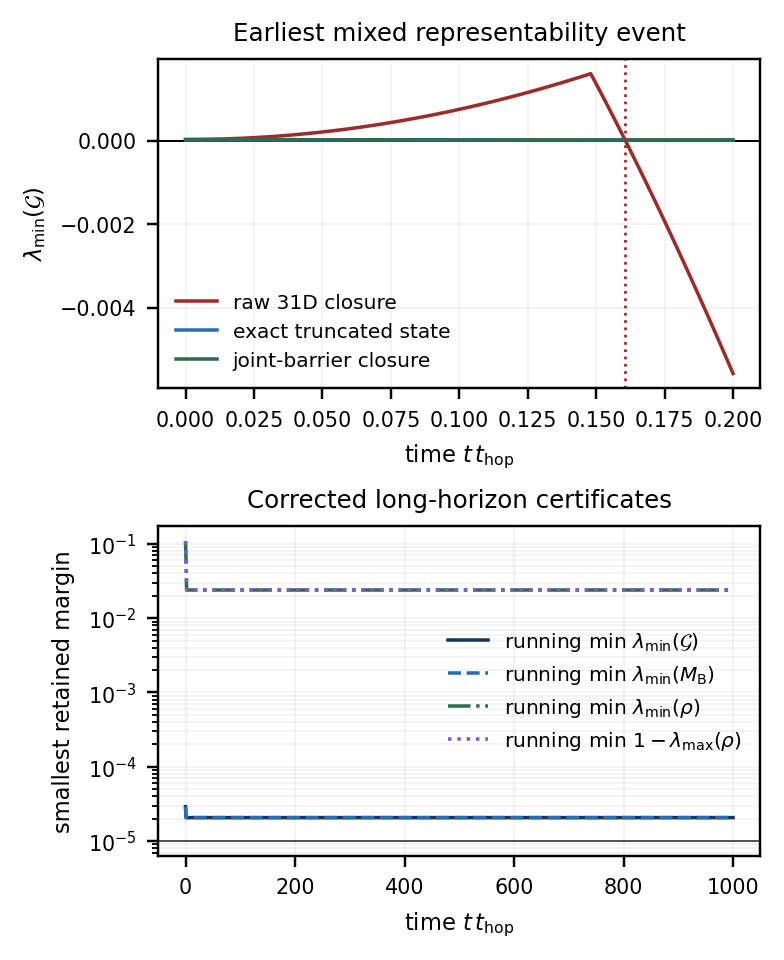
\includegraphics[width=\columnwidth]{joint_electron_phonon_addendum_evidence.pdf}

\parbox{0.96\columnwidth}{\scriptsize
\textbf{Failure and correction in the same necessary moment condition.}
The upper panel compares the raw closure, exact truncated Hamiltonian, and
joint-barrier closure near the first zero crossing.  The lower panel reports
running minima from the checkpointed corrected trajectory; the horizontal
line is the configured \(h_\star=10^{-5}\) margin.}
\end{minipage}

\segmenthead{F. Completed evidence and scientific consequence}

The checkpointed corrected trajectory used the unmodified archive closure,
the exact cutoff-16 ground-state contractions as its initial coordinate, fixed
RK4 step \(\Delta t=0.01\), and no constant initial-residual subtraction.  It
reached \(t=\RunTime\,t_{\rm hop}^{-1}\) after \(100{,}000\) steps and
\(400{,}000\) corrected right-hand-side evaluations, with
\[
\begin{aligned}
\min_t\lambda_{\min}(\mathcal G(t))&=\RunMinG,\\
\min_t\lambda_{\min}(M_{\rm B}(t))&=\RunMinB,\\
\RunMinRho
\leq\lambda_{\min}(\rho(t))
&\leq\lambda_{\max}(\rho(t))
\leq\RunMaxRho,\\
\max_{t,j}|x_j(t)|&=\RunMaxX,\\
\max_t|\operatorname{Tr}C^q(t)|&=\RunMaxTrace.
\end{aligned}
\tag{X27}
\]
Every correction solve converged.  The maximum correction norm was
\(\RunMaxCorrection\), the maximum post-pulse energy drift from \(t=4\) was
\(\RunEnergyDrift\), and the maximum absolute correction-energy flux was
\(2.64\times10^{-16}\).  The smallest corrected barrier eigenvalue was
\(-9.9994\times10^{-9}\), within the declared \(10^{-8}\) cone tolerance.

\segmenthead{G. Exact Reference Separates Admissibility from Accuracy}

The completed comparison uses the same initial contractions and the same
driven parameters \((\lambda,\gamma,V)=(1.5,0.5,1)\) for three trajectories
over \(0\leq t\leq T=4\).  The exact route propagates the full
cutoff-16 Holstein-dimer state and contracts it into
\(X_{\rm ex}(t)=(\rho_{\rm ex},B_{\rm ex},N_{\rm ex},A_{\rm ex},C_{\rm ex})\).
The raw route propagates \(f(t,x)\), and the corrected route propagates
Eq.~(X25) with fixed RK4 step \(\Delta t=0.01\).  Exact contractions enter
only after propagation as the reference against which both approximate
trajectories are measured.

For a retained matrix block
\(Y\in\{\rho,B,N,A,C\}\) and a route
\(a\in\{\mathrm r,\mathrm c\}\), define its dynamic-normalized RMS error by
\[
\begin{aligned}
D_Y^2&=\frac1T\int_0^T
\lVert Y_{\rm ex}(t)-Y_{\rm ex}(0)\rVert_{\rm F}^2\,dt,\\
\varepsilon_Y^{(a)}&=
\frac{\left[T^{-1}\int_0^T
\lVert Y_a(t)-Y_{\rm ex}(t)\rVert_{\rm F}^2\,dt\right]^{1/2}}
{D_Y}.
\end{aligned}
\tag{X28}
\]
The label \(a=\mathrm r\) denotes the raw closure and
\(a=\mathrm c\) the corrected closure.  Here \(D_Y\) is the RMS size of the
exact motion itself.  Thus
\(\varepsilon_Y=1\) means that the RMS approximation error equals the RMS
change undergone by that exact block.

Write \(g_-=\min_t\lambda_{\min}(\mathcal G(t))\),
\(b_-=\min_t\lambda_{\min}(M_{\rm B}(t))\), and
\((r_-,r_+)=(\min_t\lambda_{\min}(\rho(t)),
\max_t\lambda_{\max}(\rho(t)))\).  The physicality certificates over the
same interval are
{\scriptsize
\[
\begin{array}{@{}lccc@{}}
\toprule
\text{route}&g_-&b_-&[r_-,r_+]\\
\midrule
\text{exact}&2.8524\!\times\!10^{-5}&2.8549\!\times\!10^{-5}
&[0.08338,0.91662]\\
\text{raw}&-0.51727&-0.14777&[-0.02230,1.02230]\\
\text{corrected}&2.0637\!\times\!10^{-5}&2.0647\!\times\!10^{-5}
&[0.02395,0.97605]\\
\bottomrule
\end{array}
\tag{X29}
\]
}
The raw path first samples a negative joint eigenvalue at \(t=0.17\),
consistent with the root in Eq.~(X16).  Its correlation trace reaches
\(7.57\times10^{-2}\); the exact and corrected traces remain below
\(1.06\times10^{-15}\) and \(1.15\times10^{-16}\), respectively.

Representability is therefore restored by the joint controller.  The
blockwise accuracy comparison supplies a second, independent result:
{\scriptsize
\[
\begin{array}{@{}lrrr@{}}
\toprule
Y&\varepsilon_Y^{(\mathrm r)}&\varepsilon_Y^{(\mathrm c)}
&\max_t\lVert Y_{\rm c}-Y_{\rm ex}\rVert_{\rm F}\\
\midrule
\rho&0.6072&0.7613&0.1868\\
B&0.1076&0.2089&0.1153\\
N&6.5530&8.5389&0.3978\\
A&4.8673&4.6735&0.8951\\
C&2.5749&2.1250&0.2551\\
\bottomrule
\end{array}
\tag{X30}
\]
}
The barrier lowers the \(A\)- and \(C\)-sector RMS errors and raises the
\(\rho\)-, \(B\)-, and \(N\)-sector errors.  Its objective is the nearest
feasible velocity in the displayed coordinate metric.  Reconstruction of the
exact missing velocity would require the omitted dynamical information.  In
particular, the joint inequalities delimit which retained moments are
representable, while they do not determine the exact direction of motion
within that admissible set.  The connected mixed moment \(K\) defined in
Eq.~(X5) carries part of that missing directional information.  Consequently,
the controller can keep \(C(t)\) inside the joint cone while its trajectory
still differs from the exact contraction.

\begin{center}
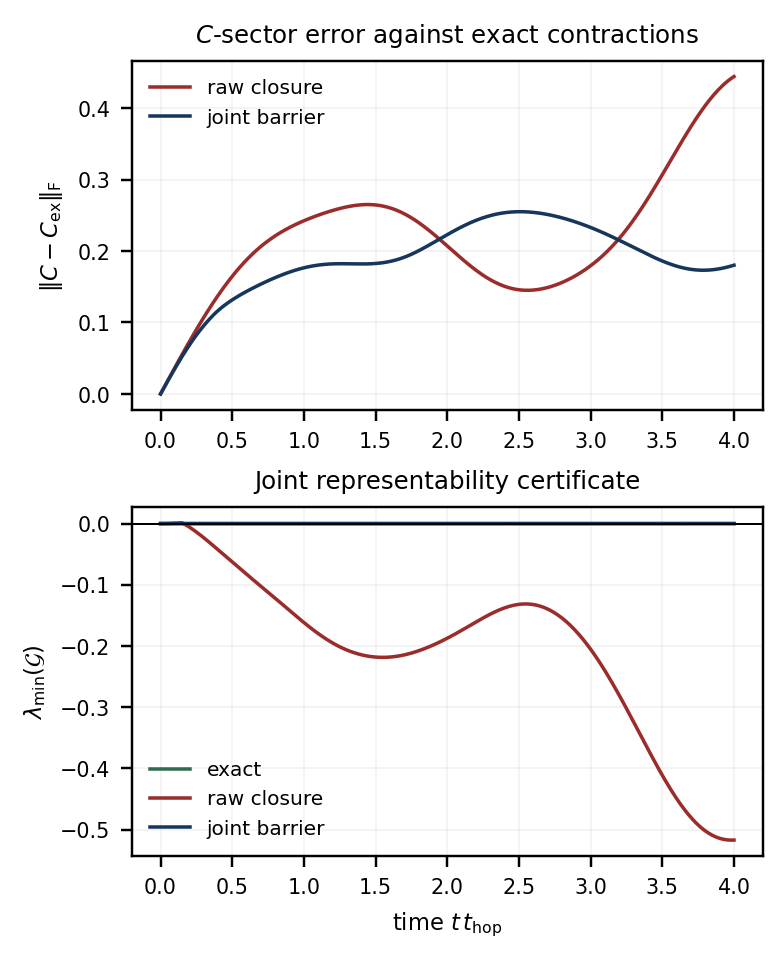
\includegraphics[width=\columnwidth]{joint_electron_phonon_accuracy_evidence.pdf}

\parbox{0.96\columnwidth}{\scriptsize
\textbf{Representability and trajectory accuracy over the driven horizon.}
The upper panel shows the accumulated \(C\)-block error against the exact
cutoff-16 contractions.  The lower panel shows that the joint barrier keeps
the corrected trajectory inside the necessary Gram cone as the raw closure
moves farther outside it.}
\end{center}

\segmenthead{H. Controller Geometry Reveals Its Actual Action}

Let \(w_{\rm e}(t)\) be the minimum-norm velocity that enforces only the
energy and trace equalities in Eq.~(X23).  The additional joint-cone action is
\[
w_{\rm g}(t)=w^\star(t)-w_{\rm e}(t),
\qquad
w^\star=w_{\rm e}+w_{\rm g}.
\tag{X31}
\]
This decomposition separates equality maintenance from the velocity inserted
to keep the Gram matrix inside its semidefinite cone.  Both terms are active
from \(t=0\).  Their largest norms are
\(\max\lVert w_{\rm e}\rVert_2=0.05939\) and
\(\max\lVert w_{\rm g}\rVert_2=0.34265\); the full correction peaks at
\(\lVert w^\star(0.62)\rVert_2=0.34552\).

For each coordinate block, let
\(P_Y:\R^{31}\to\R^{d_Y}\) extract the coordinates belonging to \(Y\).
Its integrated share of the cone action is
\[
\eta_Y=
\frac{\int_0^T\lVert P_Yw_{\rm g}(t)\rVert_2^2\,dt}
{\int_0^T\lVert w_{\rm g}(t)\rVert_2^2\,dt},
\qquad
\sum_Y\eta_Y=1,
\tag{X32}
\]
with
\[
(\eta_\rho,\eta_B,\eta_N,\eta_A,\eta_C)
=(23.37,\ 2.14,\ 0.80,\ 4.52,\ 69.18)\%.
\tag{X33}
\]
The correlation coordinates carry more than two thirds of the inserted
cone-preserving motion; the electronic density carries nearly one quarter.

The normalized weakest eigenvector \(v(t)\in\C^7\) of \(\mathcal G(t)\)
uses the operator order in Eq.~(X9).  Averaged with
\(\lVert w_{\rm g}(t)\rVert_2^2\) as the weight, its squared norm is
\(62.97\%\) electronic and \(37.03\%\) bosonic.  Its largest individual
weights are \(34.11\%\) in \(\delta\sigma_z\), \(24.51\%\) in
\(\delta\sigma_y\), and \(30.24\%\) in the two phonon-annihilation entries
together.  The electronic lower and upper cone velocities remain inward;
the joint Gram sector is the exposed barrier at every baseline sample.

\begin{center}
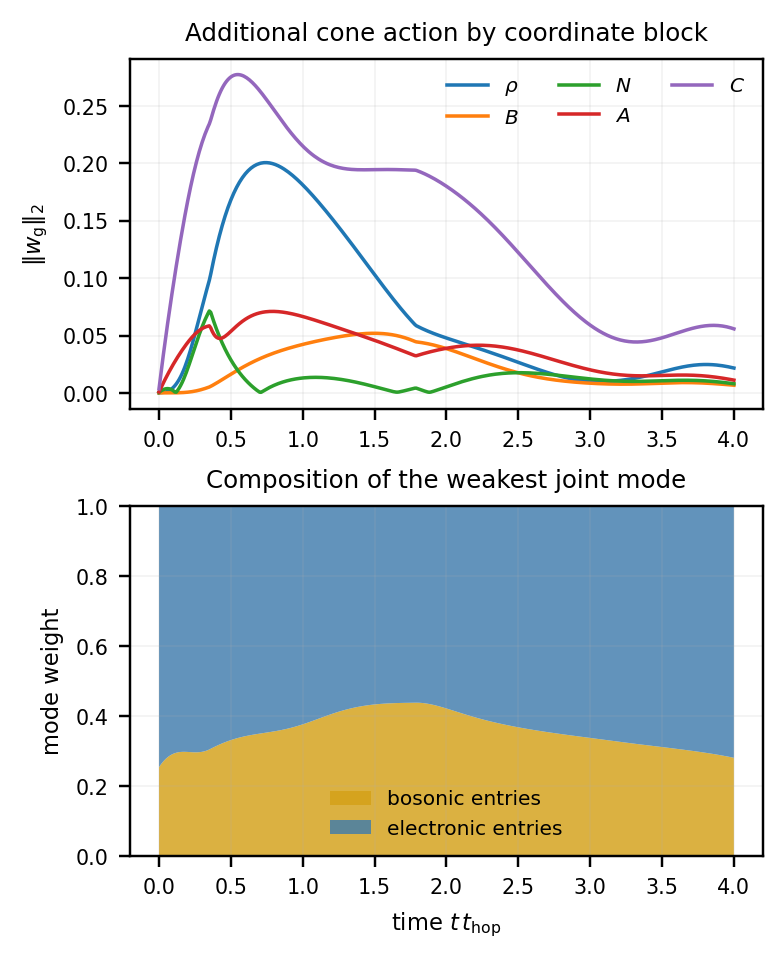
\includegraphics[width=\columnwidth]{joint_electron_phonon_mechanism_evidence.pdf}

\parbox{0.96\columnwidth}{\scriptsize
\textbf{Where the joint barrier acts.}
The upper panel resolves \(w_{\rm g}\) into the five retained coordinate
blocks.  The lower panel resolves the weakest joint-Gram eigenvector into its
bosonic and electronic operator entries.}
\end{center}

The exact trajectory supplies a direct test of whether this cone action also
reconstructs the omitted dynamics.  Let
\(r_0=f(0,x_{\rm ex}(0);V=0)\) be the undriven initial closure residual and
define the residual-subtracted derivative defect
\[
\widetilde r(t)=
f(t,x_{\rm ex}(t))-r_0-\dot x_{\rm ex}(t).
\tag{X34}
\]
The \(C\) block has RMS norm \(0.16669\) and maximum norm \(0.27431\).
It is the largest block at 400 of 401 samples; every other block has maximum
norm below \(2.32\times10^{-4}\), and the \(\rho\) defect remains at
roundoff.

At samples satisfying
\(\lVert P_C\widetilde r\rVert_2\geq0.01
\max_t\lVert P_C\widetilde r(t)\rVert_2\), compare the cone increment with
the missing exact direction \(-P_C\widetilde r\).  Their mean cosine is
\(0.374\), and every sampled cosine is positive.  The mean projection
coefficient
\[
p_C=
\frac{(P_Cw_{\rm g})^{\mathsf T}(-P_C\widetilde r)}
{\lVert P_C\widetilde r\rVert_2^2}
\tag{X35}
\]
is \(0.0956\), with mean norm ratio \(0.363\).  Hence the controller points
partly against the missing \(C\)-velocity defect and supplies only about
\(9.6\%\) of that missing direction.

\segmenthead{I. Numerical Convergence Resolves a Smaller Scale}

The time-step and cutoff tests compare trajectories at their common saved
times using the maximum blockwise Frobenius difference:
{\scriptsize
\[
\begin{array}{@{}lrr@{}}
\toprule
\text{comparison}&\max_t\Delta_C&\max_t\lVert\Delta x\rVert_2\\
\midrule
\Delta t:0.01\ \text{vs.}\ 0.005&1.3000\!\times\!10^{-6}
&3.1122\!\times\!10^{-6}\\
n_{\max}:12\ \text{vs.}\ 16&1.2377\!\times\!10^{-2}
&5.7191\!\times\!10^{-2}\\
n_{\max}:16\ \text{vs.}\ 20&3.1910\!\times\!10^{-4}
&1.6914\!\times\!10^{-3}\\
\bottomrule
\end{array}
\tag{X36}
\]
}
The first row refines the corrected integrator; the last two rows refine the
exact truncated Hamiltonian.  Cutoff 12 remains visibly coarse, and the
16-to-20 change establishes cutoff 16 as the working reference.  The corrected
\(C\)-error maximum \(0.2551\) is \(799\) times the larger numerical floor
\(3.1910\times10^{-4}\).  Time integration and phonon truncation therefore
resolve a scale far below the remaining closure error.

\segmenthead{J. Parameter Grid Preserves the Mechanism}

The robustness set is the twelve-point Cartesian product
\[
\Lambda=\{0.5,1.5\}\times\{0.25,0.5,1\}\times\{0.5,1\},
\tag{X37}
\]
whose entries are \((\lambda,\gamma,V)\).  Each point uses cutoff 16,
\(\Delta t=0.02\), and \(T=4\).  The raw joint Gram matrix becomes negative
at all twelve points; the corrected matrix remains nonnegative to the declared
cone tolerance at all twelve points.  The aggregate accuracy and correction
scales are
\[
\begin{array}{@{}lcc@{}}
\toprule
\lambda&\varepsilon_C^{(\mathrm c)}\ \text{range}
&\max_t\lVert w^\star\rVert_2\ \text{range}\\
\midrule
0.5&0.324\text{--}0.792&0.0165\text{--}0.0715\\
1.5&1.812\text{--}4.698&0.312\text{--}0.574\\
\bottomrule
\end{array}
\tag{X38}
\]
All twelve corrected \(C\)-error ratios exceed \(0.1\).  At
\((1.5,1,0.5)\), the corrected ratio \(3.494\) slightly exceeds the raw ratio
\(3.415\), establishing that cone preservation alone supplies no universal
accuracy improvement.  The strong-coupling points require both larger
interventions and retain substantially larger \(C\)-sector errors.

\segmenthead{K. Measured Scales Determine the Next Closure}

The predeclared extension gate requires a material dynamic error and a model
error separated from the numerical floor:
\[
\varepsilon_C^{(\mathrm c)}>0.1,
\qquad
\frac{\max_t\lVert C_{\rm c}-C_{\rm ex}\rVert_{\rm F}}
{\max(\delta_{\Delta t},\delta_{n_{\max}})}>10.
\tag{X39}
\]
The measured values are \(2.125\) and \(799\).  Both gates activate the model
extension already motivated by Eqs.~(X5)--(X7a).  Let
\(\mathcal R_C\) extract the fourteen independent real coordinates of
\(C=(C^0,C^1)\).  For a supplied set
\(S\subseteq\{K,P,D\}\), define
\[
\begin{aligned}
e_S(t)=\mathcal R_C\Bigl(&
 \dot C_{31}(t)+\sum_{\alpha\in S}\Delta\dot C_\alpha(t)
 -\dot C_{\rm ex}(t)\\
&-\dot C_{31}(0)-\sum_{\alpha\in S}\Delta\dot C_\alpha(0)
 +\dot C_{\rm ex}(0)\Bigr).
\end{aligned}
\tag{X40}
\]
The subtraction at \(t=0\) removes the constant initial residual.  The
remaining curve measures whether each supplied source follows the driven
change of the exact velocity.  Sequential substitution over
\(0\leq t\leq4\) gives
{\scriptsize
\[
\begin{array}{@{}lrr@{}}
\toprule
S&\operatorname{RMS}\lVert e_S\rVert_2
&\max_t\lVert e_S\rVert_2\\
\midrule
\varnothing&0.166690&0.274310\\
K&0.089345&0.137864\\
K+P&0.026160&0.038268\\
K+P+D&2.53\times10^{-5}&3.47\times10^{-5}\\
\bottomrule
\end{array}
\tag{X41}
\]
}
All three physical source terms reduce the RMS defect by a factor of
approximately \(6.58\times10^3\).  The remaining curve has the scale of the
finite-cutoff commutator remainder.

\begin{center}
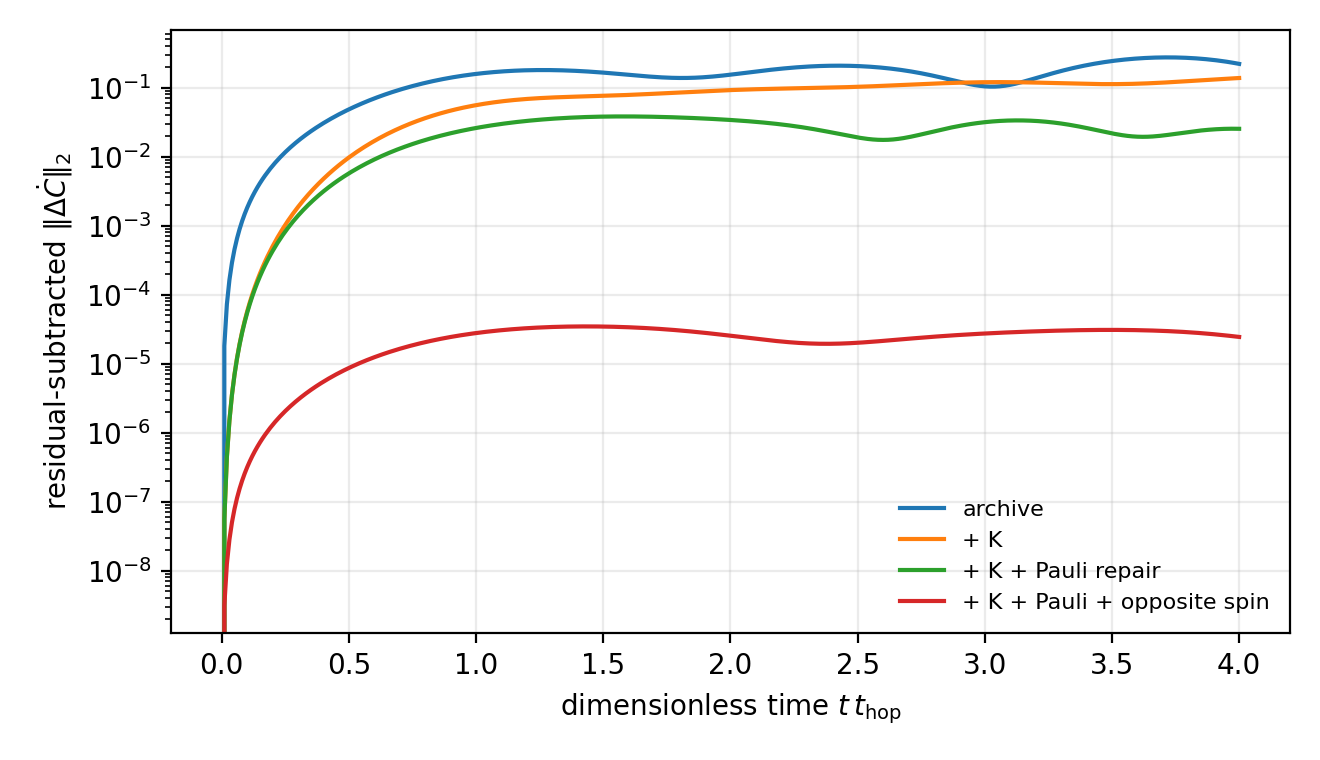
\includegraphics[width=\columnwidth]{exact_mixed_moment_closure_attribution.png}

\parbox{0.96\columnwidth}{\scriptsize
\textbf{Sequential reconstruction of the missing \(C\)-velocity.}
Each curve evaluates the archive derivative on the exact cutoff-16 trajectory
and then supplies one additional term from Eq.~(X7a).  The ordinate is the
fourteen-real-coordinate norm defined in Eq.~(X40).}
\end{center}

The cutoff sequence \(n_{\max}=12,16,20\) gives commutator-remainder changes
\[
\lVert\Delta R_{\rm cut}\rVert_{\rm F}
=(2.74\times10^{-4},\,8.38\times10^{-6},\,8.51\times10^{-8}),
\tag{X42}
\]
and the associated violations of the infinite-oscillator mode identities
decrease from \(1.8\times10^{-3}\) to \(1.1\times10^{-6}\).  Cutoff 16
therefore resolves the physical closure defect by several orders of magnitude.

\conceptbreak
\textbf{Symmetry reduction and the autonomy test.}
With \(b_\pm=(b_0\pm b_1)/\sqrt2\), the centered total mode \(b_+\)
decouples.  The exact tensors then satisfy
\[
\begin{aligned}
K^{1r}&=-K^{0r},&K^{q0}&=K^{q1},&
K^{qr}_{00}&=K^{qr}_{11}=0,\\
D^1&=-D^0,&D^0&=(D^0)^\dagger,&
\operatorname{Tr}D^0&=0.
\end{aligned}
\tag{X43}
\]
Thus the sampled \(K\) tensor reduces to four real coordinates and the
sampled \(D\) tensor reduces to three.  Appending these seven numbers to
\(x\in\R^{31}\) produces a 38-coordinate list.  An autonomous closure further
requires the Hamiltonian commutator to express the derivatives of all 38
coordinates through that same list.

That derivative test generates new moments.  Define
\(D_{\mu\nu}=\operatorname{Cov}
(\sigma^\uparrow_\mu,\sigma^\downarrow_\nu)\) and
\(\delta O=O-\langle O\rangle\).  Hopping rotates the sampled
\(D_{\mu z}\) components into the remaining \(D_{\mu\nu}\) components.
Electron--phonon coupling then produces connected
two-electron/one-phonon moments, and differentiating \(K\) produces connected
one-electron/three-phonon moments:
\[
(K,D_{\mu z})
\xrightarrow{\ \ii[H,\,\cdot\,]\ }
\left(
D_{\mu\nu},
\langle\delta O\,\delta\sigma^\downarrow\,\delta b\rangle_{\!c},
\langle\delta O\,\delta b\,\delta X\,\delta X\rangle_{\!c}
\right).
\tag{X44}
\]
The subscript \(c\) denotes the connected part remaining after all products
of lower-order moments have been removed.  Equation~(X44) is the hierarchy
obstruction: a \(K+D\) patch would place a new factorization inside the first
derivatives of its added coordinates.

\conceptbreak
\textbf{Physical content of the three model terms.}
The factorized source \(Q_0\) assigns independent statistics to the
electronic commutator and the phonon pair.  Its remainder \(K\) records how
an electronic transfer fluctuation and the instantaneous deformation of the
phonon cloud occur together.  Under the drive, their relative amplitudes and
phases evolve, so the pair of lower moments in \(Q_0\) lacks information
required by the exact correlation velocity.

The Pauli term \(P\) has a different role.  Fixed one-up-electron number
determines it algebraically from \(\rho\), as Eq.~(X7) shows.  Restoring \(P\)
therefore repairs the fermionic multiplication law at no added dynamical
dimension.  The opposite-spin covariance \(D\) records how the up-spin
one-body coherence depends on the down-spin electron's site occupation.
That conditional electronic information evolves dynamically and expands into
the full cross-spin covariance under hopping.

These mechanisms explain the ordering in Eq.~(X41).  \(K\) supplies the
largest individual velocity change, the exact Pauli algebra removes a second
systematic component, and \(D\) completes the physical source to the cutoff
floor.  Their downstream feedback alters \(\rho\), \(N\), and \(A\), thereby
carrying the initial \(C\)-velocity error into the joint moment matrix whose
eigenvalue later becomes negative.

The source-faithful candidate is a symmetry-adapted third-cumulant closure.
Its state retains the complete cross-spin covariance and the complete
relative-mode connected moment family generated at the same order as \(K\);
its terminal rule explicitly factorizes the next cumulant order.  The exact
audit in Eq.~(X41) supplies the red test for that construction.  Exact
contractions remain offline reporting data, and the joint Gram barrier remains
a separate representability safeguard applied to the enlarged raw velocity.

\newpage
\par\smallskip
\noindent{\color{green}\rule{\columnwidth}{1.1pt}}\par\vspace{-1pt}
{\small
\noindent\textbf{\color{green}Resolved correction and established limit}
\par\smallskip\color{black}
The long run establishes that the joint 31-coordinate barrier can keep the
archive closure inside the retained electron--phonon moment constraints through
\(t=1000\).  The matched exact run establishes that this admissible trajectory
still carries a converged strong-coupling accuracy error concentrated in
\(C\).  The controller's dominant action lies in the \(C\) and \(\rho\)
coordinates and only partially aligns with the missing exact \(C\) velocity.
\par}
\vspace{1pt}\noindent{\color{navy!35}\rule{\columnwidth}{0.35pt}}

\newpage
\par\smallskip
\noindent{\color{green}\rule{\columnwidth}{1.1pt}}\par\vspace{-1pt}
{\small
\noindent\textbf{\color{green}Next physics-model construction}
\par\smallskip\color{black}
The exact operator audit reconstructs that missing velocity from \(K\), the
Pauli-algebra repair, and opposite-spin covariance to the finite-cutoff floor.
The complete symmetry-adapted third-cumulant state, followed by an explicit
next-order factorization, is therefore the next physics-model construction.
\par}
\vspace{1pt}\noindent{\color{navy!35}\rule{\columnwidth}{0.35pt}}

\clearpage
\segmenthead{L. Coordinate Basis and Validation Chain}

The 31 correction numbers in Eq.~(X17) are coefficients of the standard real
basis of the propagated coordinate space.  For
\(j,k\in\{0,\ldots,30\}\), define
\[
(e_j)_k=\delta_{jk},
\qquad
w=\sum_{j=0}^{30}w_je_j\in\R^{31}.
\tag{X45}
\]
Substitution of one basis vector \(e_j\) into Eqs.~(X17)--(X20) produces one
fixed matrix-velocity pattern.  Linearity then gives
{\small
\[
\begin{aligned}
&(\Delta\dot\rho,\Delta\dot B,\Delta\dot N,
  \Delta\dot A,\Delta\dot C)(w)\\
&\hspace{8mm}=\sum_{j=0}^{30}w_j
(\Delta\dot\rho,\Delta\dot B,\Delta\dot N,
  \Delta\dot A,\Delta\dot C)(e_j).
\end{aligned}
\tag{X46}
\]
}
Thus each \(w_j\) scales the entry pattern generated by the corresponding
state coordinate.  The optimization objective is exactly
\[
\tfrac12\lVert w\rVert_2^2
=\tfrac12\sum_{j=0}^{30}w_j^2.
\tag{X47}
\]
The Frobenius size of the lifted matrix velocity has a different coordinate
weighting:
{\small
\[
\begin{aligned}
&\lVert\Delta\dot\rho\rVert_{\rm F}^2
+\lVert\Delta\dot B\rVert_2^2
+\lVert\Delta\dot N\rVert_{\rm F}^2
+\lVert\Delta\dot A\rVert_{\rm F}^2
+\sum_q\lVert\Delta\dot C^q\rVert_{\rm F}^2\\
&\hspace{27mm}=w^{\mathsf T}Ww,
\qquad W\neq I_{31}.
\end{aligned}
\tag{X48}
\]
}
The matrix \(W\in\R^{31\times31}\) is the fixed coordinate metric induced by
the matrix lift.  Repeated conjugate entries, symmetric copies, and the
one-half factors in Eqs.~(X17) and (X20) determine its weights.  Thus
\(w^{\mathsf T}I_{31}w=\lVert w\rVert_2^2\) measures the Euclidean size of
the independent coordinate coefficients, while \(w^{\mathsf T}Ww\) measures
the Frobenius size of their lifted matrix-entry patterns.  Hence Eq.~(X23)
minimizes the
independent real coordinate changes.  A Frobenius-minimum correction would
replace the objective by \(w^{\mathsf T}Ww/2\).

\conceptbreak
\textbf{Archive-equation transcription.}
The first check compared two independently written calculations of the same
retained derivative.  For 100 seeded random state--time pairs,
\[
\begin{aligned}
r_{13}(t,x)
&=f_{13}(t,x)-\Pi_{13}F(t,\mathcal E_{13}(x)),\\
r_{13}&\simeq0
\quad(\mathrm{atol}=\mathrm{rtol}=2\times10^{-15}).
\end{aligned}
\tag{X49}
\]
The scalar route \(f_{13}\) was handwritten from the specialized component
equations; the matrix route reconstructed the same state, evaluated the
archive matrix equations, and extracted the same thirteen slopes.  Agreement
at roundoff checks signs, conjugations, factors, and index placement on every
shared coordinate.

The 31-coordinate route is the composition
\(f=\Pi\circ F\circ\mathcal E\).  Its randomized checks therefore tested the
maps surrounding \(F\): 100 coordinate round trips obeyed
\(\mathcal R(\mathcal E(x))=x\) at tolerances
\(2\times10^{-16}\), and 100 matrix velocities had unrepresented normal
residual below \(3\times10^{-14}\).  These results establish that the chosen
31 coordinates reconstruct their matrix tuple and contain every matrix
direction generated in the tested dimer sector.

\conceptbreak
\textbf{Exact-reference comparison.}
Transcription agreement asks whether two representations evaluate the same
archive equations.  Accuracy asks whether those equations give the same local
motion as the truncated Holstein Hamiltonian.  At each saved exact state,
Eq.~(X2) evaluated
\[
r(t_k)=f(t_k,x_{\rm ex}(t_k))
-\mathcal R\dot X_{\rm ex}(t_k),
\qquad
\dot X_{\rm ex}=\ii\langle[H,\widehat X]\rangle .
\tag{X50}
\]
The commutator supplies the exact contracted derivative at \(t_k\); no
finite difference between neighboring trajectory samples enters Eq.~(X50).
The 401-point driven comparison localized the evolving defect in \(\dot C\),
and the substitutions \(K\), \(K+P\), and \(K+P+D\) in Eq.~(X41) reduced its
RMS norm from \(0.166690\) to \(2.53\times10^{-5}\).

\segmenthead{M. Lift, Optimizer, and Trajectory Checks}

The analytic correction lift was checked as a directional derivative.  With
\(\varepsilon=10^{-7}\), a supplied real direction \(w\), and the current
state \(x\), centered differences gave
{\small
\[
\begin{aligned}
&\frac{\mathcal G(\mathcal E(x+\varepsilon w))
-\mathcal G(\mathcal E(x-\varepsilon w))}{2\varepsilon}
=\Delta\dot{\mathcal G}(w)+O(\varepsilon^2),\\
&\frac{E(\mathcal E(x+\varepsilon w))
-E(\mathcal E(x-\varepsilon w))}{2\varepsilon}
=\nabla_xE(x)^{\mathsf T}w+O(\varepsilon^2).
\end{aligned}
\tag{X51}
\]
}
The analytic and finite-difference arrays agreed to relative and absolute
tolerances \(10^{-8}\).  Separate structural checks verified
\(\Delta\dot\rho=\Delta\dot\rho^\dagger\),
\(\operatorname{Tr}\Delta\dot\rho=0\), the Hermitian/symmetric block
relations in Eq.~(X19), and the trace action in Eq.~(X20).

The constrained solve was then tested at states chosen to expose its active
conditions.  At the exact cutoff-16 initial contractions, the raw joint
barrier was below \(-2\times10^{-3}\).  The cutting-plane solve returned a
joint barrier above \(-10^{-9}\), correlation-trace velocity below
\(10^{-12}\), and correction-energy flux below \(2\times10^{-11}\).  A
direct eigenvalue-constrained solve produced the same correction norm to
relative tolerance \(2\times10^{-7}\).  At the recorded
\(t=28.57\) state, the restricted thirteen-control problem was infeasible;
the full 31-coordinate problem converged, satisfied all three marginal
barriers above \(-10^{-9}\), and used nonzero correlation controls.  These
checks isolate feasibility, equality preservation, and the minimum-norm solve
from the subsequent time integration.

\conceptbreak
\textbf{A correction is solved at every RK4 stage.}
For any provisional stage time \(\tau_r\) and state \(y_r\), Eq.~(X23)
supplies a fresh correction \(w_r^\star=w^\star(\tau_r,y_r)\).  The stage
velocity and its coordinate increment are
\[
k_r=f(\tau_r,y_r)+w_r^\star,
\qquad
hk_r=h f(\tau_r,y_r)+h w_r^\star.
\tag{X51a}
\]
Thus the correction enters the derivative sampled by RK4, and multiplication
by the step duration \(h\) converts that rate into its contribution to the
state increment.  Define
\(f_{\rm c}(t,x)=f(t,x)+w^\star(t,x)\), where \(w^\star(t,x)\) is obtained
from Eq.~(X23) after reconstructing the matrices at that stage state.  The
accepted pair \((t_n,x_n)\) supplies the starting time and coordinate state,
and \(h\) is the duration of one step.  Each
\(k_i\in\R^{31}\) is a corrected instantaneous velocity evaluated at one
provisional stage pair.  Its product \(hk_i\) is therefore a coordinate
increment.  One fixed step is
{\small
\[
\begin{aligned}
k_1&=f_{\rm c}(t_n,x_n),\\
k_2&=f_{\rm c}(t_n+h/2,x_n+hk_1/2),\\
k_3&=f_{\rm c}(t_n+h/2,x_n+hk_2/2),\\
k_4&=f_{\rm c}(t_n+h,x_n+hk_3),\\
x_{n+1}&=x_n+\frac h6(k_1+2k_2+2k_3+k_4).
\end{aligned}
\tag{X52}
\]
}
The vectors \(x_n+hk_1/2\), \(x_n+hk_2/2\), and \(x_n+hk_3\) are provisional
stage states.  The second and third stages share the time \(t_n+h/2\) and
generally have different states, so their corrected velocities may differ.
The weighted increment
\(h(k_1+2k_2+2k_3+k_4)/6\) approximates the integral of the coordinate
velocity across this single step.  Every occurrence of \(f_{\rm c}\) performs
a fresh reconstruction and a fresh constrained solve.  The four stage pairs
are solver-internal evaluations; \(x_{n+1}\) is the stored endpoint sample.
Thus the
\(t=1000\) run used \(100{,}000\) stored steps and \(400{,}000\) corrected
right-hand-side evaluations.  Every internal correction solve converged.

The short first-exit test propagated the raw route through
\(t=0.2\), where the sampled joint minimum fell below \(-10^{-3}\), and the
corrected RK4 route through the same interval, where the joint minimum stayed
above \(10^{-5}\) and the two correlation traces remained zero to
\(2\times10^{-12}\).  The long trajectory then supplied Eq.~(X27).
Refining \(h=0.01\) to \(0.005\) changed the state at \(t=2\) by
\(1.18\times10^{-6}\); the trajectory comparison in Eq.~(X36) and the
cutoff sequence \(12,16,20\) place the numerical scale below the measured
closure defect.  The twelve-point grid in Eq.~(X37) repeated the raw-cone and
corrected-cone comparison across the tested parameter set.

\tracebox{green}{What each layer establishes}
Directional finite differences in Eq.~(X51) validate the analytic matrix lift
and energy covector locally: their first-order changes agree with independent
centered differences.  They leave global cone preservation and closure
accuracy unproved.

The cutting-plane and direct constrained optimizers return the same correction
norm at the tested active states and satisfy the barrier, trace, and
energy conditions.  This comparison validates the constrained minimum-norm
solve at those states; it leaves future-stage feasibility and Hamiltonian
accuracy unproved.

RK4 step refinement measures sensitivity to the numerical time step, and the
short and long trajectories test accumulated constraint preservation.  These
tests leave the moment closure and the infinite-cutoff Hamiltonian limit
unproved.

The exact contracted commutator in Eq.~(X50) tests local closure accuracy, and
the matched exact trajectory tests accumulated observable accuracy.  The
cutoff sequence measures truncation sensitivity of that reference; it leaves
the selected Gram inequalities as necessary, rather than sufficient,
conditions for a complete quantum state.
\closetracebox

\tracebox{navy}{Representability stabilization and closure accuracy}
Constraint satisfaction places the approximate trajectory inside the selected
electronic, joint-Gram, trace, and energy conditions.  Exact
truncated-Hamiltonian contractions separately determine whether its velocity
and observables follow the reference dynamics.  The joint correction
stabilizes admissibility.  The remaining \(C\)-sector defect measures the
inaccurate moment closure and persists until its missing dynamical information
is modeled.
\closetracebox

\segmenthead{N. Reconstruction Checklist}

\begin{itemize}[label=\(\square\)]
  \item Can I construct \(e_j\), substitute it into Eqs.~(X17)--(X20), and
  recover the complete lift by Eq.~(X46)?
  \item Can I explain why \(\lVert w\rVert_2\) measures independent coordinate
  coefficients and why the lifted Frobenius metric contains \(W\)?
  \item Can I state which part of Eq.~(X49) was independently transcribed and
  which part of the 31-coordinate test checks composition and tangency?
  \item Can I reconstruct Eq.~(X50) and explain why the commutator derivative
  tests closure accuracy without a trajectory finite difference?
  \item Can I derive both centered differences in Eq.~(X51) and identify the
  analytic quantities they test?
  \item Can I name every inequality and equality in Eq.~(X23), including
  \(\beta=5\) and \(h_\star=10^{-5}\)?
  \item Can I write all four lines of Eq.~(X52) and identify where the fresh
  optimization occurs?
  \item Can I separate the claims supported by derivative parity, exact
  reference, optimizer tests, trajectory refinement, and cutoff refinement?
\end{itemize}

\segmenthead{O. Post-Reading Mastery Quiz (Exit Quiz)}

For each question, select the strongest claim and record the decisive reason.

\textbf{Q1.} The residual in Eq.~(X49) is roundoff-level at 100 random
state--time pairs.  What follows?
\begin{enumerate}[label=\Alph*.]
  \item The archive closure reproduces the exact truncated-Hamiltonian
  trajectory at all later times.
  \item The handwritten scalar and reconstructed matrix routes assign the same
  thirteen retained derivatives to the tested states.
  \item The joint Gram matrix remains positive semidefinite under every
  propagated parameter choice.
  \item The minimum Euclidean correction also minimizes the lifted Frobenius
  norm.
\end{enumerate}

\textbf{Q2.} Why does Eq.~(X50) use the Hamiltonian commutator?
\begin{enumerate}[label=\Alph*.]
  \item It differentiates the exact retained expectation values at one state
  without dividing the difference of two saved samples.
  \item It projects the approximate trajectory onto the exact Hilbert-space
  state after every RK4 stage.
  \item It converts the 31 real correction coordinates into a Frobenius-orthogonal
  matrix basis.
  \item It enforces the semidefinite inequalities before the exact reference is
  propagated.
\end{enumerate}

\textbf{Q3.} Which objective would select the smallest lifted Frobenius
velocity under the same constraints?
\begin{enumerate}[label=\Alph*.]
  \item \(\tfrac12w^{\mathsf T}Ww\).
  \item \(\tfrac12\sum_j|\lambda_j(\mathcal G)|\).
  \item \(\tfrac12\lVert f(t,x)\rVert_2^2\).
  \item \(\tfrac12\lVert x+w\rVert_2^2\).
\end{enumerate}

\textbf{Q4.} At the provisional state \(x_n+hk_1/2\), what supplies \(k_2\)?
\begin{enumerate}[label=\Alph*.]
  \item The correction solved at \(x_n\), reused with coefficient one-half.
  \item A fresh matrix reconstruction and a fresh Eq.~(X23) solve at the
  provisional state.
  \item A projection of the accepted endpoint back into the joint Gram cone.
  \item The exact contracted derivative from Eq.~(X50).
\end{enumerate}

\Needspace{16\baselineskip}
\textbf{Q5.} Which result establishes that the remaining \(C\)-sector error
is a model-closure error resolved above the numerical floor?
\begin{enumerate}[label=\Alph*.]
  \item The round-trip identity \(\mathcal R(\mathcal E(x))=x\) by itself.
  \item The joint barrier remaining nonnegative through the short first-exit
  test by itself.
  \item The exact-reference defect together with step and cutoff refinement in
  Eqs.~(X36), (X41), and (X42).
  \item The equality \(\operatorname{Tr}\Delta\dot\rho=0\) by itself.
\end{enumerate}

\segmenthead{P. Advisor-Defense Transfer and Repair}

Answer each prompt aloud as a compact technical argument.  Begin with the
governing map or equation, follow the mechanism into the numerical operation,
and close with the physical claim that the calculation supports.  The
correction coordinates are
\[
\begin{aligned}
w^\star(\tau,y)
&=\bigl(w_0^\star,\ldots,w_{30}^\star\bigr)\in\R^{31},\\
f_{\rm c}(\tau,y)
&=f(\tau,y)+w^\star(\tau,y).
\end{aligned}
\tag{X53}
\]
Here \(\tau\) is one Runge--Kutta stage time, \(y\in\R^{31}\) is its
provisional coordinate state, and \(w^\star(\tau,y)\) is the minimum-norm
correction to the archive velocity at that stage.  Its entries use the same
coordinate order as \(x\).  Eqs.~(X17)--(X21) lift those independent real
coefficients into the matrix velocities needed by the constraints.

\textbf{A1. Time propagation from the integral.}
Interpret Eq.~(X52) as the propagation of one vector from \(x_n\) to
\(x_{n+1}\).  Identify the four stage pairs at which the velocity is sampled,
explain why \(k_i\) has the same 31 components as \(x\) but represents a rate
of change, and show where multiplication by \(h\) converts that rate into a
coordinate increment.  Then explain why \(k_2\) and \(k_3\) generally differ
despite sharing the time \(t_n+h/2\), and identify the accepted, stored
endpoint.

\textbf{A2. One corrected right-hand-side evaluation.}
At a stage pair \((\tau,y)\), write the complete causal chain
\[
y\xrightarrow{\mathcal E}X(y)
\longrightarrow f(\tau,y)
\longrightarrow w^\star(\tau,y)
\longrightarrow f_{\rm c}(\tau,y)
\longrightarrow k_i.
\]
State what each arrow computes, which reconstructed matrices enter the
constraints, and why the optimization must be solved again at every
provisional stage state.  Then compare the implemented velocity update
\(f_{\rm c}=f+w^\star\) with a direct state replacement
\(y\leftarrow y+w^\star\), and trace how the implemented correction reaches
the accepted state through the RK4 integral.

\textbf{A3. The correction basis and its structured matrix lift.}
Using the standard basis \(e_j\in\R^{31}\), expand
\[
w^\star=\sum_{j=0}^{30}w_j^\star e_j
\longmapsto
\bigl(\Delta\dot\rho,\Delta\dot B,\Delta\dot N,
\Delta\dot A,\Delta\dot C,\Delta\dot{\mathcal G}\bigr)(w^\star).
\]
Explain how one coefficient produces one fixed matrix-entry pattern through
Eqs.~(X17)--(X21), why Hermiticity, symmetry, and trace structure survive the
lift, and why the matrix-valued codomain is required to impose the PSD
constraints.  Explicitly distinguish this full 31-coordinate controller from
a reduced correction vector that would first require a separate map into
\(\R^{31}\).

\textbf{A4. The constrained minimum-norm correction.}
Restate Eq.~(X23) with \(w\) as the optimization variable.  Define
\(\beta=5\) as the recovery rate, \(h_\star=10^{-5}\) as the retained
eigenvalue margin.  Explain the roles of the three PSD inequalities for
\(\rho\), \(I_2-\rho\),
and \(\mathcal G\), followed by the correlation-trace and energy equalities.
State precisely what \(w^\star=0\) establishes about the raw stage velocity,
and distinguish that local feasibility statement from exactness of the moment
closure.  Finally compare the implemented Euclidean objective
\(\lVert w\rVert_2^2/2\) with the lifted Frobenius objective
\(w^{\mathsf T}Ww/2\).

\textbf{A5. Evidence sufficient for an advisor-facing claim.}
Suppose the claim is: ``The archive equations were transcribed correctly, the
raw closure leaves the representable moment set, the joint controller supplies
the intended minimum-norm feasible velocity, and the stabilized closure still
differs from exact truncated-Hamiltonian dynamics.''  Assign each clause to
the evidence that supports it: random-state derivative parity, round-trip and
tangency checks, the first joint-Gram eigenvalue crossing, directional
finite-difference checks of the lift and energy row, agreement between the
cutting-plane and direct constrained solves, short first-exit propagation,
long-time propagation, RK4 step refinement, phonon-cutoff refinement, and the
exact commutator/trajectory comparison.  State the evidentiary limit of each
test as part of the argument.

\textbf{A6. Sensitivity of one exposed mode.}
For the normalized eigenvector \(v\) in Eq.~(X25a), define
\(a_j=v^\dagger\Delta M(e_j)v\).  Explain why \(a_j\) is a scalar sensitivity
rather than an eigenvalue, derive
\(\phi_v(w)=\lambda+\sum_j a_jw_j\), and interpret the sign and magnitude of
\(a_j\) as the effect of the \(j\)-th unit correction on the failing mode.

\textbf{A7. From one mode inequality to the full PSD condition.}
Equation~(X26) constrains one normalized direction \(v\), whereas
Eq.~(X26c) quantifies over every direction \(z\).  Explain why a correction
that repairs the current \(v\) may expose a different minimizing eigenvector,
and reconstruct the diagonalize--add constraint--resolve cycle.

\textbf{A8. Fixed-number trace restoration.}
Use Eqs.~(X14) and (X23a) to connect fixed particle number to
\(s=\operatorname{Tr}C^q=0\).  Explain why \(s(0)=0\) remains zero and why a
small numerical trace error decays as \(e^{-\beta t}\).

\newpage
\segmenthead{Detachable Solutions}

\textbf{Q1: B.}
Equation~(X49) compares two implementations of the same archive derivative on
the shared thirteen coordinates.  Exact trajectory agreement requires the
separate Hamiltonian comparison in Eq.~(X50).

\textbf{Q2: A.}
The Heisenberg equation evaluates the derivative of each contracted operator
expectation at the current exact state.  Neighboring saved values therefore
play no role in the derivative defect.

\newpage
\textbf{Q3: A.}
Equation~(X48) expresses the lifted Frobenius norm as \(w^{\mathsf T}Ww\).
The implemented objective \(w^{\mathsf T}w/2\) uses the displayed coordinate
metric.

\textbf{Q4: B.}
The second line of Eq.~(X52) calls \(f_{\rm c}\) at the provisional state;
the definition of \(f_{\rm c}\) includes a new Eq.~(X23) solve there.

\textbf{Q5: C.}
The exact-reference comparison measures the physical derivative and trajectory
defect, and the two refinements bound the numerical scale beneath it.  A
representation identity or cone certificate alone supplies no accuracy bound.

\end{document}
